%Im Folgenden werden die Einzelheiten zum Betrieb des Prototypen beschrieben und dienen gleichzeitig als Dokumentation für die zukünftige Entwicklung und Administration des Systems.

\subsection{Softwarevoraussetzungen}
Für den Betrieb des Steckerbots werden folgende Komponenten vorausgesetzt:

\begin{itemize}
\item git
\item Docker
\item Docker-Compose
\item Internet-Verbindung
\end{itemize}

Das bevorzugte Betriebssystem ist Linux, da dieses im Serverbereich weit verbreitet ist und auch während der Entwicklung durchgängig eingesetzt wurde. Der Betrieb auf anderen Betriebssystemen ist durch den Einsatz von Docker-Containern nicht ausgeschlossen, wurde aber nicht getestet.
Zur Weiterentwicklung des Bots sind NodeJS, npm, ein MySQL-Client, das coffeescript-Paket und yeoman nötig.

\subsection{Einstellung der Slack-Plattform}
Da der Slackbot als virtueller Nutzer in Slack laufen soll, benötigt dieser eine Verbindung zu entsprechenden Workspace in Slack. Dazu ist vom Administrator oder Entwickler ein Slack-Token zu generieren.
Dieser Slack-Token kann durch Hinzufügen einer neuen Hubot-Konfiguration generiert werden.\footnote{\url{https://my.slack.com/apps/A0F7YS25R-bots}} Dabei muss der anlegende Nutzer bereits ein Konto bei Slack haben und in dem Workspace registriert sein, in welchem der Bot laufen soll.
Nach dem in \autoref{img:hubot-int} erscheinenden Dialog zur Eingabe des Namens für den Bot wird ein eindeutiger Token generiert und angezeigt. Dieser wird für die weitere Installation benötigt und beginnt mit \texttt{xoxb-}.

\begin{figure}[H]
    \centering
    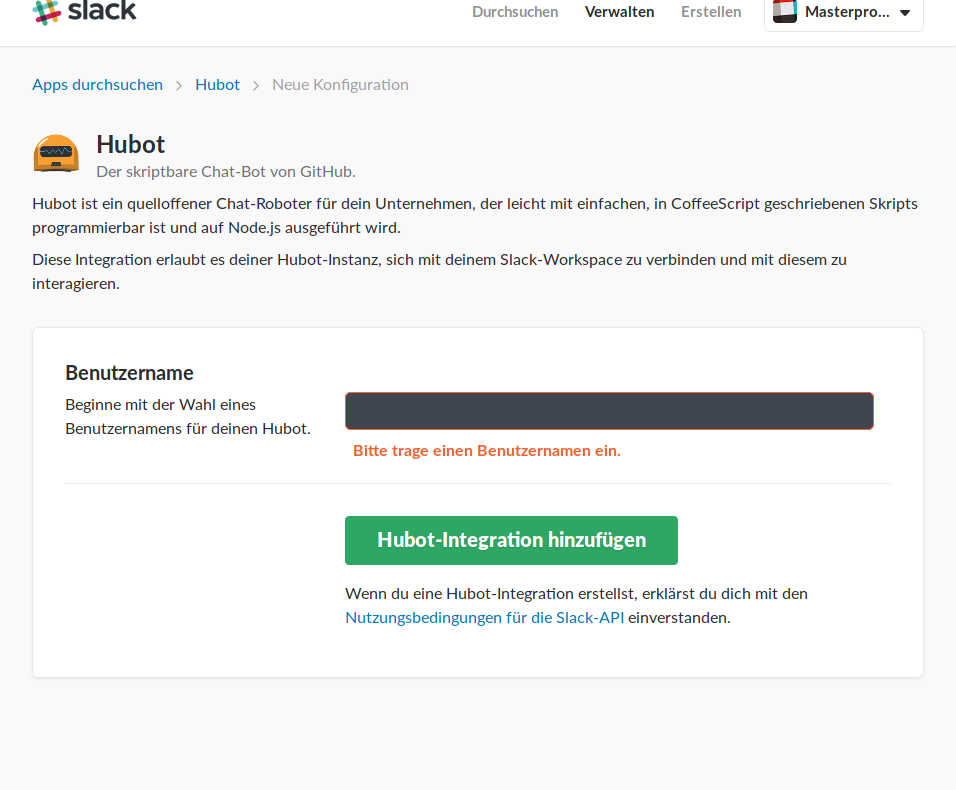
\includegraphics[width=0.8\textwidth]{img/hubot-int.png}
    \caption{Seite zum Anlegen einer neuen Bot-Konfiguration}
    \label{img:hubot-int}
\end{figure}

\subsection{Starten der lokalen Umgebung}
Nach Abruf des Projekts\footnote{\url{https://github.com/ohli/steckerbot}}
(über \texttt{git clone} oder Herunterladen des Archivs) befindet sich der Quellcode im Ordner \textit{docker} mit folgenden Dateien:

\begin{verbatim}
bin/
db-data/
node_modules/
scripts/
abfragen.sql
docker-compose.yml
Dockerfile
external-scripts.json
generate_config.sh
package.json
\end{verbatim}

Die Umgebung wird dynamisch aus zwei Docker-Containern aufgebaut, welche mittels docker-compose verknüpft werden. Alle vom Standard abweichenden Einstellungen werden über die \texttt{steckerbot.env} definiert. Diese kann über den Aufruf der \texttt{generate\_""config.sh} generiert werden. Beim Aufruf wird automatisch ein Passwort für den MySQL-Rootnutzer erzeugt sowie weitere Umgebungsvariablen gesetzt. Dies ist nur für Testzwecke vorgesehen und kann im produktiven Betrieb durch ein selbst gewähltes Passwort ersetzt werden. Aktuell liegen die Passwörter im Klartext in der .env-Datei vor, was durch den Einsatz von z.B. Docker Secrets\footnote{\url{https://docs.docker.com/engine/reference/commandline/secret/}} vermieden werden sollte.

In den Ordnern bin, node\_modules und scripts befinden sich Dateien des Hubot-Frameworks. db-data enthält SQL-Dateien die zur Laufzeit zum initialisieren der Datenbank genutzt werden.

Die ausgelieferte Standardkonfiguration kann nach Anlegen der .env-Datei über die folgenden Befehle gestartet werden:

\texttt{docker-compose build}

\texttt{docker-compose up}

Dies startet und initialisiert zuerst einen lokalen MySQL-Container und verbindet anschließend den Hubot-Container mit dieser. Nun sollte der zuvor im Slack angelegte Bot als \enquote{online} erscheinen und auf erste einfache Befehle antworten.

Zum Stoppen der Container ist im gleichen Ordner \texttt{docker-compose down} einzugeben bzw. die laufende Log-Ausgabe mittels \texttt{Ctrl+C} zu beenden.

\subsection{Initialisieren der Datenbank}
Die im vorherigen Unterabschnitt angelegte Datenbank muss zu Beginn noch mit Daten gefüllt werden. Im Gegensatz zum Hubot-Container dessen Zustand nur beim Aufruf von \texttt{docker-compose build} geändert wird, speichert der MySQL-Container die Datenbanken in einem persistenten Docker-Volume \texttt{db-data} ab.

Zum Anlegen neuer Nutzer wird folgender Vorgang empfohlen:

\begin{enumerate}
    \item ermitteln der IP-Adresse des MySQL-Containers mittels \texttt{docker inspect termindatenbank}
    \item Verbinden eines MySQL-Clients wie z.B. MySQL Workbench\footnote{\url{https://www.mysql.com/de/products/workbench/}} mit der IP des MySQL-Containers
    \item Anlegen der gewünschten Daten in die bereits bestehenden Tabellen
\end{enumerate}

Die angelegten Daten können anschließend mit den .sql-Dateien aus dem Ordner sql-tests getestet werden.

\subsection{Beispielbefehle}

Folgende Befehle wurden im Prototyp implementiert (\autoref{tab:protcmd}):

\begin{table}[h!]
    \centering
    \begin{tabularx}{\textwidth}{|X|X|X|}
        \hline
        \textbf{Befehl} & \textbf{Beschreibung} & \textbf{Antwort} (Beispiel) \\
        \hline
        ping & testet Verbindung des Bots & PONG \\
        \hline
        hilfe & Zeigt Liste der Befehle an & siehe diese Tabelle \\
        \hline
        füge mich der Datenbank hinzu als Paula Panzer & fügt Nutzer initial mit dem Namen 'Paula Panzer' der Datenbank hinzu & \texttt{Nutzer} wurde in die Datenbank als Paula Panzer eingefügt \\
        \hline
        Wann ist die nächste Schicht? & zeigt nächste verfügbare Schicht an & Die nächste Schicht ist: Sommerfest 2018-04-08 13:00:00 \\
        \hline
        Trag mich ein & trägt Nutzer in zuvor angezeigte Schicht ein & Ich habe dich in die Schicht eingetragen \\
        \hline
        Danke & beendet Konversation \& Kontext der Schicht & Gern geschehen \\
        \hline
    \end{tabularx}
    \caption{Befehle des Bot-Prototyps}
    \label{tab:protcmd}
\end{table}


\subsection{Besonderheiten und Best Practices}

Im Verlauf der Entwicklung des Bots traten stellenweise unerwartete Probleme auf, deren Lösungsansätze für zukünftige Weiterentwicklungen von Nutzem sein dürften.

\textbf{Änderung des Botnamens}: Der Name des Bots steht zusammen mit anderen Metadaten in der \texttt{package.json} im docker-Ordner.

\textbf{Mangelnde Schreibberechtigung im Hubot-Container}: die Hubot-Skripte müssen unter dem Nutzer Hubot laufen und sollten direkt in den Container gemounted werden.

\textbf{Änderung der NodeJS Version}: die NodeJS-Version ist zur Wahrung der Stabilität explizit in der docker-compose.yml-Datei anzugeben.


